\documentclass[12pt,a4paper,utf8]{ctexart}
\usepackage{ctex,amsmath,amssymb,subfig,cite,graphicx,diagbox,fontspec,fancyhdr,geometry}
\usepackage[ntheorem]{empheq}
\usepackage{enumitem,fullpage,cleveref,cellspace,listings,color,framed}
\definecolor{gray}{rgb}{0.5,0.5,0.5}
\definecolor{dkgreen}{rgb}{.068,.578,.068}
\definecolor{dkpurple}{rgb}{.320,.064,.680}

%set Fortran styles
\lstset{
    frameround=tftf,
    language=Fortran,
    keywords={SELECT,PROGRAM,PRINT,STOP,END,WRITE,INTEGER,REAL,COMPLEX,CHARACTER,LOGICAL,READ,FORMAT,IMPLICIT,PARAMETER,DATA,EQUIVALENCE,TYPE,PAUSE,CONTINUE,CYCLE,EXIT,IF,SELECT,DO,ALLOCATE,DEALLOCATE,WHERE,FORALL,SUBROUTIHNE,CALL,RETURN,FUNCTION,COMMON,BLOCK DATA,SAVE,INTERFACE,CONTAIN,MODULE,USE,PUBLIC,PRIVATE,ENTRY,OPEN,INQUIRE,CLOSE,NAMELIST,POINTER,NULLFY,REWIND,BACKSPACE,ENDFILE
    },
    basicstyle=\small\ttfamily,
    numbers=left,
    numberstyle=\small,
    keywordstyle=\color{blue}\bfseries,
    commentstyle=\color{dkgreen},
    stringstyle=\color{dkpurple},
    backgroundcolor=\color{white},
    tabsize=2,
    showspaces=false,
    showstringspaces=false,
    breaklines=true,
    frame=trBL,
}
\CTEXsetup[format+={\raggedright}]{section}
\setlength{\parindent}{2em}
\geometry{
    textwidth=138mm,
    textheight=215mm,
    left=27mm,
    right=27mm,
    top=25.4mm,
    bottom=25.4mm,
    headheight=2.17cm,
    headsep=4mm,
    footskip=12mm,
    heightrounded,
}
\pagestyle{fancy}
\lhead{\textsl{2021秋-计算物理A}}
\chead{}
\rhead{\textsl{PB19020634-于浩然}}
\lfoot{}
\cfoot{\thepage}
\rfoot{}

\begin{document}
\begin{center}
    {\LARGE\textbf{计算物理作业十三}}\\
    \textrm{于浩然}~~~~~~\textrm{PB19020634}~~~~~~\textrm{2021.12.06}
\end{center}
\section{作业题目}

用Metropolis-Hasting抽样方法计算积分:
\begin{equation}
    I = \int _0 ^{\infty} (x-\alpha \beta)^2 f(x) \textrm{d}x = \alpha \beta ^2
\end{equation}
\begin{equation}
    f(x) = \frac{1}{\beta \Gamma(\alpha)} \left( \frac{x}{\beta}\right)^{\alpha
    - 1} \exp (-x/\beta)
\end{equation}

设积分的权重函数分别为:$p(x) = f(x)$和$p(x)=(x-\alpha \beta)^2 f(x)$. 

给定参数$\alpha, \beta$,并用不同的$\gamma$值,分别计算积分,讨论计算精度和效率.
\section{算法简介}
\subsection{Markov链}

当满足条件$p_n(x_1,\cdots,x_n;t_1,\cdots,t_n) = p_n(x_1,\cdots,x_n;t_1+\Delta
t,\cdots,t_n +\Delta
t)$时,称随机过程是平稳的,即时间的起点选取没有影响,时,称随机过程是平稳的,即时间的起点选取没有影响,时间
序列仅表示$x$取值的先后.

我们称一个平稳的随机序列是Markov的,如果某一时刻$x$取值的条件几率独立于上一时刻之前
所有$x$值的话. Markov链的极限分布与初始分布的选择无关,仅决定于转移概率.
分布概率和转移概率分别用$p,W$来表示,达到平衡时有如下关系:
\begin{equation}
    p_i = \sum_j p_jW_{ji}
\end{equation}

\subsection{平稳态的主方程}

平稳态主方程可以写为
\begin{equation}
    \frac{p(x)}{p(x')} = \frac{W(x'\rightarrow x)}{W(x\rightarrow x')}
\end{equation}

上式中已经考虑了到达平衡态与时间无关. 此即统计力学中的细致平衡解.
将变量$x,x'$分别用下标$i,j$替换,则方程(4)写为
\begin{equation}
    p_iW_{ij}=p_jW_{ji}
\end{equation}
\subsection{Metropolis-Hasting抽样规则}

Metropolis-Hasting抽样规则中,建议分布和接受几率均取非对称,接受几率根据
待满足的几率分布$p$而定. 

由细致平衡条件,
\begin{equation}
    \frac{p_j}{p_i} = \frac{W_{ij}}{W_{ji}} =
    \frac{T_{ij}A_{ij}}{T_{ji}A_{ji}},\quad A_{ij}= \min \left\{1,
    \frac{p_jT_{ji}}{p_iT_{ij}}\right\}
\end{equation}
\begin{equation}
    W_{ij} = 
    \begin{cases}
        T_{ij}\qquad  &,p_jT_{ji}>p_iT_{ij} \\
        T_{ij}(p_j/p_i)\quad  &,p_jT_{ji}<p_iT_{ij}
    \end{cases}
\end{equation}

式中$i,j$不相同,$W_{ii}$须通过归一性求出. 根据建议分布$T$进行初始抽样,
$T(x\rightarrow x')$最好是和$p$形状相近的任意条件概率分布. 不妨取$T_{ij} =
T(x\rightarrow x')=T(x')=0.5\exp\{-x'/\gamma\}$并设$x_0=1$,具体抽样方法如下:

假设已经产生了$n$个抽样点$x_1,x_2,\cdots,x_n$,由所设的建议分布$T_{ij}$给出试探解
$x'$.
\begin{enumerate}
    \item[(1)] 做抽样$x'=-\gamma \ln R$, $R$是(0,1)区间上均匀分布的随机数;
    \item[(2)] 计算$r= \frac{p_jT_{ji}}{p_iT_{ij}}$,

        具体到积分1:
        \begin{equation}
            r = \left( \frac{x'}{x_n}\right)^{\alpha-1}\exp\{-(x'-x_n)/\beta\}
            \exp\{(x'-x_n)/\gamma\}
        \end{equation}
        积分2:没有意义. 这将在后面进行阐释. 
        \begin{equation}
            x_{n+1} = 
            \begin{cases}
                x' \quad&,if~R<\min(1,r)\\
                x_n \quad&,if~ R>\min(1,r)
            \end{cases}
        \end{equation}

    \item[(3)] 
        积分1:
        \begin{equation}
            I= \frac{1}{N} \sum _{i=1} ^N (x_i-\alpha \beta)^2
        \end{equation}

        积分2:

        前面的方法总会得到相同的结果1,Metropolis-Hasting方法不能计算积分.
        若要考虑对求积分方法作修改,
        序列$\{x\}$反映了$x$按$p(x)$分布的情况,积分$\int _0 ^{\infty} p(x)
        \textrm{d}x$可由$p(x)$与$x$轴所围面积来反映,这相当于没有权重计算积分的情形,
        在考虑Metropolis方法的本题中便不予考虑. 
\end{enumerate}
\section{编程实现}

不妨取参数$\alpha = 3,\beta = 2$,积分理论值为12. 求积分1时,$\gamma$从0到25之间取,
步进为0.1;
求积分2的子程序已编写,与积分一大同小异,但由于其没有意义故没有放在主程序中输出结果.
用FORTRAN90进行编程实现,具体程序见附录. 

\section{计算结果}
\begin{itemize}
    \item $p(x) = f(x)$

        积分值随$\gamma$值变化的情况如下:
        \begin{figure}[h]
            \centering
            \subfloat[全部值]{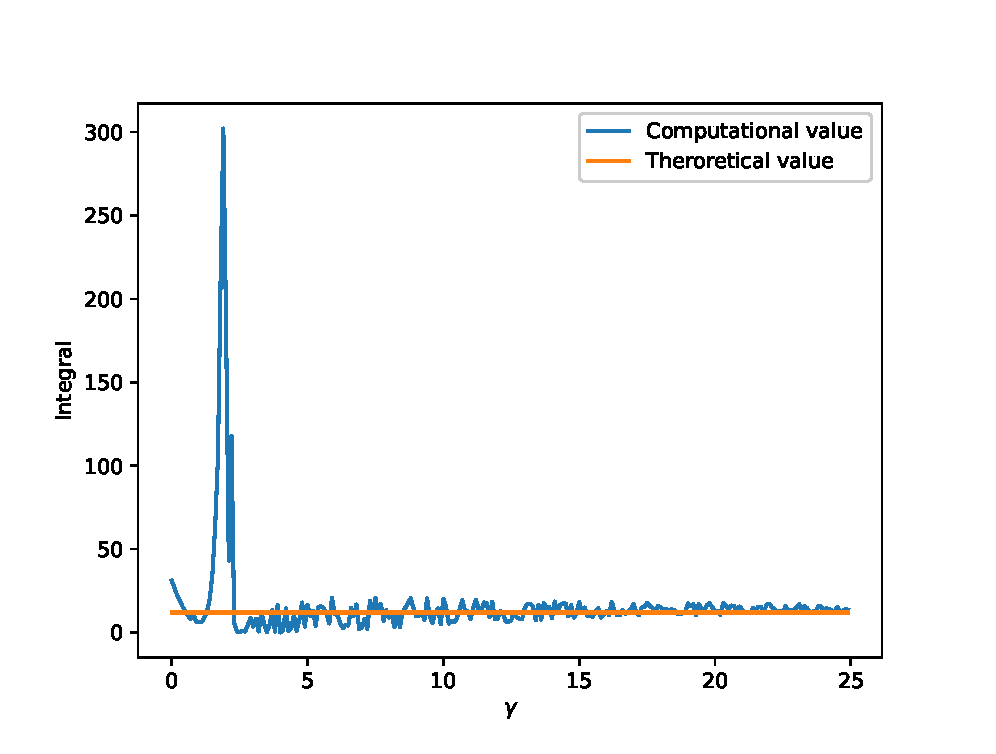
\includegraphics[width=0.5\textwidth]{integral1_1.eps}}
            \hfill
            \subfloat[去除大偏差部分]{\includegraphics[width=0.5\textwidth]{integral1_2.eps}}
            \caption{积分计算值随$\gamma$变化情况(1)}
        \end{figure}

        图中看出,在$\gamma=2$附近有一极大的偏离,将$\gamma<5$的数据剔除后得到图1(b).
        作误差分布图如下:

        \begin{figure}[!h]
            \centering
            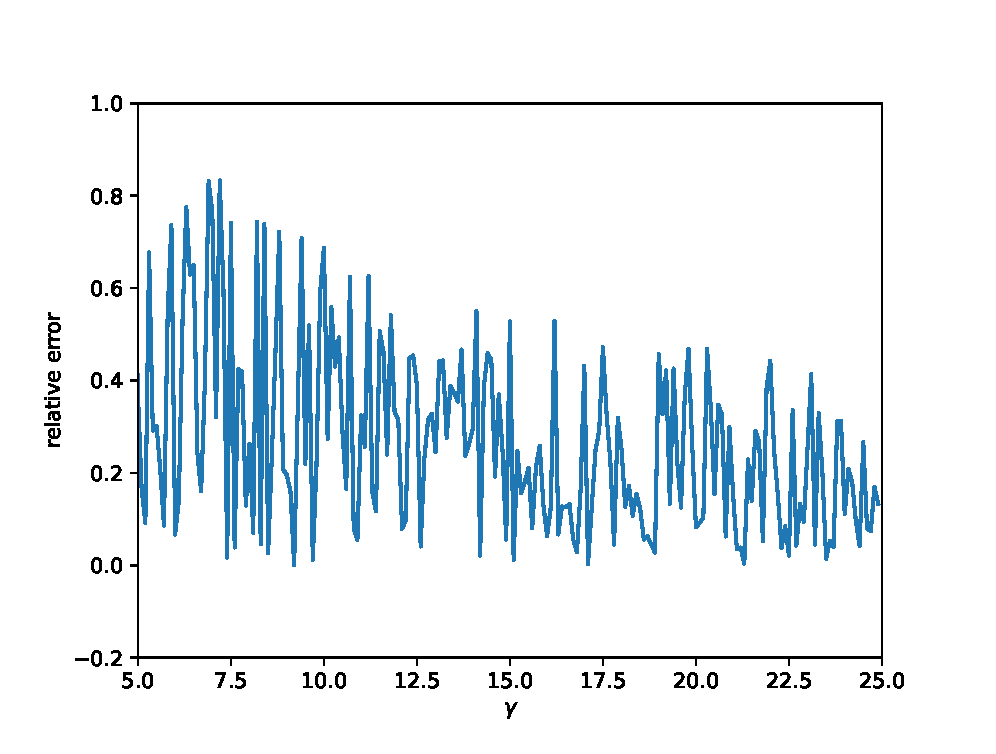
\includegraphics[width=0.8\textwidth]{error1.eps}
            \caption{积分1误差分布图}
        \end{figure}

        观察图像得到,在研究区间内误差随着$\gamma$增大而减小,
        当$\gamma > 20$时误差情况较好,约在$30\%$以内.
    \item $p(x) = (x-\alpha \beta)^2 f(x)$

        此时积分的计算无意义,在上一节中解释过,故不列出结果.
\end{itemize}
\section{结论}

本次作业实现了Metropolis-Hasting抽样方法计算积分,得到了具有一定误差的结果,
当$\gamma$为适当值时积分计算更加精确,推测这是由于初始分布的形状与实际分布比较接近.
并发现了当除去权重函数的被积
函数为常数时这一方法将不再有效,总得到无意义的结果“1”.
推测这是由于在使用权重函数时仅顾及了分布而丢失了它的部分信息,使得积分的计算不可能.
要想精确地计算积分,需要恰当选取被积函数和MC权重函数;若想要提高计算效率(积分收敛到
精确值的速度),则需要谨慎选取初始建议分布的形式,如本题中的$\gamma$选取.

\section{源代码}
\subsection{FORTRAN90代码}
\begin{framed}
\begin{lstlisting}[language=Fortran]
MODULE Metropolis
IMPLICIT NONE

CONTAINS
SUBROUTINE Sample1(a, b, gam, num)
    REAL(KIND=8) ,INTENT(IN) :: gam
    REAL(KIND=8) :: rand(num), integral
    REAL(KIND=8) xt, x(0:num), r, seed
    INTEGER(KIND=4), INTENT(IN) :: a, b, num
    INTEGER(KIND=4) :: i
    x(0) = 1
    integral = 0
    CALL RANDOM_NUMBER(seed) 
    ! 用FORTRAN自带的随机数生成器生成16807生成器的种子
    CALL Schrage(num, int(2147483647 * seed), rand)
    DO i = 1, num
        xt = - gam * LOG(rand(i))
        r = (xt / x(i-1))**(a - 1) * EXP(-(xt - x(i-1)/b)) * EXP((xt - x(i-1))/gam)
        IF(rand(i) < MIN(1.0, r)) THEN
            x(i) = xt 
        ELSE
            x(i) = x(i-1) ! 若建议未通过,仍保留结果与上一步相同. 
        END IF
        integral = real(integral * (i-1)) / i + (x(i) - a * b)**2 / i 
        ! 按步求平均值,以防止求和溢出
    END DO
    OPEN (1, ACCESS='append', file='integral.dat')
    WRITE (1, *) integral
    CLOSE(1)
    print *, integral
END SUBROUTINE Sample1

SUBROUTINE Sample2(a, b, gam, num)
    REAL(KIND=8) ,INTENT(IN) :: gam
    REAL(KIND=8) :: rand(num), integral
    REAL(KIND=8) xt, x(0:num), r, seed
    INTEGER(KIND=4), INTENT(IN) :: a, b, num
    INTEGER(KIND=4) :: i
    x(0) = 1
    integral = 0
    CALL RANDOM_NUMBER(seed) 
    ! 用FORTRAN自带的随机数生成器生成16807生成器的种子
    CALL Schrage(num, int(2147483647 * seed), rand)
    DO i = 1, num
        xt = - gam * LOG(rand(i))
        r = (xt / x(i-1))**(a - 1) * (xt - a * b)**2 / (x(i-1) - a * b)**2&
            * EXP(-(xt - x(i-1)/b)) * EXP((xt - x(i-1))/gam)
        IF(rand(i) < MIN(1.0, r)) THEN
            x(i) = xt 
        ELSE
            x(i) = x(i-1) ! 若建议未通过,仍保留结果与上一步相同. 
        END IF
        integral = real(integral * (i-1)) / i + 1.0 / i 
        ! 直接求抽样结果x的平均值
    END DO
    OPEN (1, ACCESS='append', file='integral_2.dat')
    WRITE (1, *) integral
    CLOSE(1)
    print *, integral
END SUBROUTINE Sample2
END MODULE Metropolis

SUBROUTINE Schrage(num, z0, rand)
    !Schrage随机数生成器子程序,将均匀随机数序列存放在数组rand中
    IMPLICIT NONE
    INTEGER(KIND=4) :: N = 1, num
    INTEGER :: m = 2147483647, a = 16807, q = 127773, r = 2836, In(num), z0
    REAL(KIND=8), INTENT(INOUT) :: rand(num)
    In(1) = z0 !将传入值z0作为种子
    rand(1) = REAL(In(1))/m
    DO N = 1, num - 1
        In(N + 1) = a * MOD(In(N), q) - r * INT(In(N) / q)
        IF (In(N + 1) < 0) THEN !若值小于零,按Schrage方法加m
            In(N + 1) = In(N + 1) + m
        END IF
        rand(N + 1) = REAL(In(N + 1))/m !得到第N+1个随机数
    END DO
END SUBROUTINE Schrage

PROGRAM MAIN
    USE Metropolis
    IMPLICIT NONE
    INTEGER(KIND=4) :: i
    REAL(KIND=8) :: gam
    DO i = 1, 250
        gam = 0.1 * i
        CALL Sample1(3, 2, gam, 1000000)
    END DO
END PROGRAM MAIN
\end{lstlisting}
\end{framed}
\subsection{python绘图脚本代码}
\begin{framed}
\begin{lstlisting}[language=python]
import numpy as np
import matplotlib.pyplot as plt
import math
import matplotlib as mpl
mpl.use('TkAgg')

plt.rcParams['savefig.dpi'] = 300
plt.rcParams['figure.dpi'] = 300

#积分1
x = np.arange(0, 25, 0.1)
y = np.loadtxt('integral.dat')
y1 = np.abs(y - 12) / 12
plt.xlabel('$\gamma$')
plt.ylabel('Integral')
plt.plot(x, y)
y0 = 12 * np.ones(250)
plt.plot(x, y0)
plt.legend(['Computational value', 'Theroretical value'])
plt.savefig('integral1_1.eps')

plt.ylim(-5, 30)
plt.xlim(5, 25)
plt.savefig('integral1_2.eps')
plt.show()

plt.xlim(5, 25)
plt.ylim(-0.2, 1)
plt.plot(x, y1)
plt.xlabel('$\gamma$')
plt.ylabel('relative error')
plt.savefig('error1.eps')
plt.show()
\end{lstlisting}
\end{framed}
\end{document}


